\documentclass[usenames,dvipsnames]{beamer}
\usepackage{../../shared/styles/custom}
\usepackage{../../shared/styles/conventions}

% Define a new counter for pop quizzes
%\newcounter{popquiz}

\newcommand{\E}{\mathbb{E}}


\title{Gradient Descent: The Foundation of Machine Learning Optimization}
\subtitle{From Taylor Series to Modern Deep Learning}
\date{\today}
\author{Nipun Batra and the teaching staff}
\institute{IIT Gandhinagar}
\begin{document}
  \maketitle

  \begin{frame}{Table of Contents}
    \tableofcontents
  \end{frame}

  \section{Mathematical Foundations}
  
  \begin{frame}{The Big Picture: Why Optimization Matters}
    \begin{itemize}[<+->]
        \item \textbf{Core ML Problem:} Find best parameters $\vtheta^*$ for our model
        \item \textbf{Examples everywhere:}
        \begin{itemize}
            \item Linear regression: Minimize $(y - \mX\vtheta)^2$
            \item Neural networks: Minimize classification/regression loss
            \item Logistic regression: Minimize cross-entropy loss
        \end{itemize}
        \item \textbf{Challenge:} Most ML problems have no closed-form solution
        \item \textbf{Solution:} Iterative optimization algorithms
    \end{itemize}
    
    \pause
    \begin{keypointsbox}
    Gradient descent is the workhorse of modern machine learning!
    \end{keypointsbox}
  \end{frame}

  \begin{frame}{Gradient Intuition: Climbing Mountains}
    \textbf{Imagine you're hiking in dense fog and want to reach the valley:}
    
    \begin{itemize}[<+->]
        \item You can only feel the slope beneath your feet
        \item \textbf{Strategy:} Always step in the steepest downhill direction
        \item \textbf{Gradient} = Direction of steepest \textcolor{red}{uphill} (ascent)
        \item \textbf{Negative gradient} = Direction of steepest \textcolor{blue}{downhill} (descent)
    \end{itemize}
    
    \pause
    \begin{center}
    \includegraphics[scale=0.8]{../../maths/assets/mathematical-ml/figures/contour-x_squared_plus_y_squared_quiver-with-gradient.pdf}
    \end{center}
    
    \pause
    \textbf{Mathematical definition:} $\nabla f(x, y) = \begin{bmatrix} \frac{\partial f}{\partial x} \\ \frac{\partial f}{\partial y} \end{bmatrix}$
  \end{frame}

  \section{Taylor Series: The Mathematical Foundation}

  \begin{frame}{Why Taylor Series? The Local Approximation}
    \begin{definitionbox}{The Key Insight}
    If we can't solve $\min f(\vx)$ exactly, let's approximate $f(\vx)$ locally and optimize that!
    \end{definitionbox}
    
    \pause
    \textbf{Taylor series expansion around point $\vx_0$:}
    \begin{align}
        f(\vx) &= f(\vx_0) + \nabla f(\vx_0)^T(\vx-\vx_0) + \frac{1}{2}(\vx-\vx_0)^T\nabla^2 f(\vx_0)(\vx-\vx_0) + \ldots
    \end{align}
    
    \pause
    \begin{itemize}[<+->]
        \item \textbf{Zero-order:} $f(\vx) \approx f(\vx_0)$ (just the function value)
        \item \textbf{First-order:} $f(\vx) \approx f(\vx_0) + \nabla f(\vx_0)^T(\vx-\vx_0)$ (linear approximation)
        \item \textbf{Second-order:} Includes curvature via Hessian $\nabla^2 f(\vx_0)$
    \end{itemize}
  \end{frame}

  \begin{frame}{Taylor Series: Concrete Example}
    \textbf{Let's approximate} $f(x) = \cos(x)$ \textbf{around} $x_0 = 0$:
    
    \begin{itemize}[<+->]
        \item $f(0) = \cos(0) = 1$
        \item $f'(0) = -\sin(0) = 0$
        \item $f''(0) = -\cos(0) = -1$
        \item $f'''(0) = \sin(0) = 0$
        \item $f^{(4)}(0) = \cos(0) = 1$
    \end{itemize}
    
    \pause
    \textbf{Taylor approximations:}
    \begin{align}
        \text{0th order:} \quad &f(x) \approx 1\\
        \text{2nd order:} \quad &f(x) \approx 1 - \frac{x^2}{2}\\
        \text{4th order:} \quad &f(x) \approx 1 - \frac{x^2}{2} + \frac{x^4}{24}
    \end{align}
    
    \pause
    \begin{alertbox}{Key Insight}
    Higher-order terms give better approximations, but first-order is often sufficient for optimization!
    \end{alertbox}
  \end{frame}

  \begin{frame}{From Taylor Series to Gradient Descent}
    \textbf{Goal:} Find $\Delta \vx$ such that $f(\vx_0 + \Delta \vx) < f(\vx_0)$
    
    \pause
    \textbf{Using first-order Taylor approximation:}
    \begin{align}
        f(\vx_0 + \Delta \vx) &\approx f(\vx_0) + \nabla f(\vx_0)^T \Delta \vx
    \end{align}
    
    \pause
    \textbf{To minimize, we need:} $\nabla f(\vx_0)^T \Delta \vx < 0$
    
    \pause
    \begin{examplebox}{Vector Geometry Insight}
    For vectors $\mathbf{a}$ and $\mathbf{b}$: $\mathbf{a}^T\mathbf{b} = |\mathbf{a}||\mathbf{b}|\cos(\theta)$
    \\\textbf{Minimum when:} $\cos(\theta) = -1$ (opposite directions!)
    \end{examplebox}
    
    \pause
    \textbf{Optimal choice:} $\Delta \vx = -\alpha \nabla f(\vx_0)$ where $\alpha > 0$
    
    \pause
    \begin{definitionbox}{Gradient Descent Update Rule}
    $$\vx_{\text{new}} = \vx_{\text{old}} - \alpha \nabla f(\vx_{\text{old}})$$
    \end{definitionbox}
  \end{frame}

  \stepcounter{popquiz}
  \begin{frame}{Pop Quiz \#\thepopquiz: Taylor Series Understanding}
    \begin{popquizbox}{\thepopquiz}
    Given $f(x) = x^2 + 2$ and expansion point $x_0 = 2$:
    
    \textbf{Questions:}
    \begin{enumerate}
        \item What is $f(x_0)$?
        \item What is $f'(x_0)$?
        \item Write the first-order Taylor approximation
        \item If we take a step $\Delta x = -0.1 \cdot f'(x_0)$, what is our new $x$?
    \end{enumerate}
    \end{popquizbox}
  \end{frame}

  \section{Gradient Descent Algorithm}

  \begin{frame}{The Gradient Descent Algorithm}
    \begin{definitionbox}{Gradient Descent}
    An iterative first-order optimization algorithm for finding local minima of differentiable functions
    \end{definitionbox}
    
    \pause
    \textbf{Algorithm:}
    \begin{enumerate}[<+->]
        \item \textbf{Initialize:} $\vtheta_0$ (random or educated guess)
        \item \textbf{For} $t = 0, 1, 2, \ldots$ until convergence:
        \begin{itemize}
            \item Compute gradient: $\vg_t = \nabla f(\vtheta_t)$
            \item Update parameters: $\vtheta_{t+1} = \vtheta_t - \alpha \vg_t$
            \item Check convergence: $|\vg_t| < \epsilon$ or $|f(\vtheta_{t+1}) - f(\vtheta_t)| < \epsilon$
        \end{itemize}
    \end{enumerate}
    
    \pause
    \begin{keypointsbox}
    \textbf{Key Properties:}
    \begin{itemize}
        \item First-order method (uses gradients, not Hessians)
        \item Greedy/local search (follows steepest descent)
        \item Guaranteed to converge for convex functions
    \end{itemize}
    \end{keypointsbox}
  \end{frame}

  \begin{frame}{The Learning Rate: Your Step Size}
    \textbf{The learning rate} $\alpha$ \textbf{controls how big steps we take}
    
    \begin{itemize}[<+->]
        \item \textbf{Too small:} Slow convergence, many iterations needed
        \item \textbf{Too large:} May overshoot minimum, unstable
        \item \textbf{Way too large:} Divergence! Function values increase
    \end{itemize}
    
    \pause
    \textbf{Let's see this visually...}
  \end{frame}

  \begin{frame}{Learning Rate: Too Small ($\alpha = 0.01$)}
    \textbf{Convergence is slow but stable}
    \begin{center}
    \includegraphics[scale=0.8]{../../maths/assets/mathematical-ml/figures/gd-lr-0.01.pdf}
    \end{center}
    
    \begin{alertbox}{Problem}
    Takes many iterations to reach the minimum. Computationally expensive!
    \end{alertbox}
  \end{frame}

  \begin{frame}{Learning Rate: Just Right ($\alpha = 0.1$)}
    \textbf{Good balance: Fast and stable convergence}
    \begin{center}
    \includegraphics[scale=0.8]{../../maths/assets/mathematical-ml/figures/gd-lr-0.1.pdf}
    \end{center}
    
    \begin{keypointsbox}
    This is often the sweet spot for many problems!
    \end{keypointsbox}
  \end{frame}

  \begin{frame}{Learning Rate: Too Large ($\alpha = 0.8$)}
    \textbf{Fast but may overshoot}
    \begin{center}
    \includegraphics[scale=0.8]{../../maths/assets/mathematical-ml/figures/gd-lr-0.8.pdf}
    \end{center}
    
    \begin{alertbox}{Warning}
    Quick convergence but risk of instability. Watch out for oscillations!
    \end{alertbox}
  \end{frame}

  \begin{frame}{Learning Rate: Disaster ($\alpha = 1.01$)}
    \textbf{Divergence! Function values explode}
    \begin{center}
    \includegraphics[scale=0.8]{../../maths/assets/mathematical-ml/figures/gd-lr-1.01.pdf}
    \end{center}
    
    \begin{alertbox}{Disaster Zone}
    The algorithm diverges. Always monitor your loss curves!
    \end{alertbox}
  \end{frame}

  \section{Gradient Descent for Linear Regression}

  \begin{frame}{Linear Regression: Our First Real Application}
    \textbf{Problem:} Learn $y = \theta_0 + \theta_1 x$ from data
    
    \begin{center}
    \begin{tabular}{|c|c|}
        \hline
        \textbf{x} & \textbf{y} \\
        \hline
        1 & 1 \\
        2 & 2 \\
        3 & 3 \\
        \hline
    \end{tabular}
    \end{center}
    
    \pause
    \textbf{Cost Function (Mean Squared Error):}
    $$\MSE(\theta_0, \theta_1) = \frac{1}{n}\sum_{i=1}^n (y_i - \hat{y}_i)^2 = \frac{1}{n}\sum_{i=1}^n (y_i - \theta_0 - \theta_1 x_i)^2$$
    
    \pause
    \textbf{Goal:} $(\theta_0^*, \theta_1^*) = \argmin_{\theta_0, \theta_1} \MSE(\theta_0, \theta_1)$
  \end{frame}

  \begin{frame}{Computing Gradients for Linear Regression}
    \textbf{We need:} $\nabla \MSE = \begin{bmatrix} \frac{\partial \MSE}{\partial \theta_0} \\ \frac{\partial \MSE}{\partial \theta_1} \end{bmatrix}$
    
    \pause
    \textbf{Let's compute each partial derivative:}
    
    \begin{align}
        \frac{\partial \MSE}{\partial \theta_0} &= \frac{2}{n}\sum_{i=1}^n (y_i - \theta_0 - \theta_1 x_i)(-1)\\
        &= -\frac{2}{n}\sum_{i=1}^n \epsilon_i
    \end{align}
    
    \pause
    \begin{align}
        \frac{\partial \MSE}{\partial \theta_1} &= \frac{2}{n}\sum_{i=1}^n (y_i - \theta_0 - \theta_1 x_i)(-x_i)\\
        &= -\frac{2}{n}\sum_{i=1}^n \epsilon_i x_i
    \end{align}
    
    where $\epsilon_i = y_i - \hat{y}_i$ is the residual.
  \end{frame}

  \begin{frame}{Gradient Descent: Step-by-Step Example}
    \textbf{Initial values:} $\theta_0 = 4, \theta_1 = 0$, \textbf{Learning rate:} $\alpha = 0.1$
    
    \pause
    \textbf{Iteration 1:}
    \begin{itemize}[<+->]
        \item Predictions: $\hat{y}_1 = 4, \hat{y}_2 = 4, \hat{y}_3 = 4$
        \item Errors: $\epsilon_1 = 1-4 = -3, \epsilon_2 = 2-4 = -2, \epsilon_3 = 3-4 = -1$
        \item $\frac{\partial \MSE}{\partial \theta_0} = -\frac{2}{3}(-3-2-1) = 4$
        \item $\frac{\partial \MSE}{\partial \theta_1} = -\frac{2}{3}(-3 \cdot 1 - 2 \cdot 2 - 1 \cdot 3) = 6.67$
        \item $\theta_0 = 4 - 0.1 \times 4 = 3.6$
        \item $\theta_1 = 0 - 0.1 \times 6.67 = -0.67$
    \end{itemize}
    
    \pause
    \textbf{New parameters:} $(\theta_0, \theta_1) = (3.6, -0.67)$
  \end{frame}

  \begin{frame}{Visual Journey: Gradient Descent in Action}
    \textbf{Let's watch gradient descent navigate the loss landscape:}
    
    \begin{center}
    \only<1>{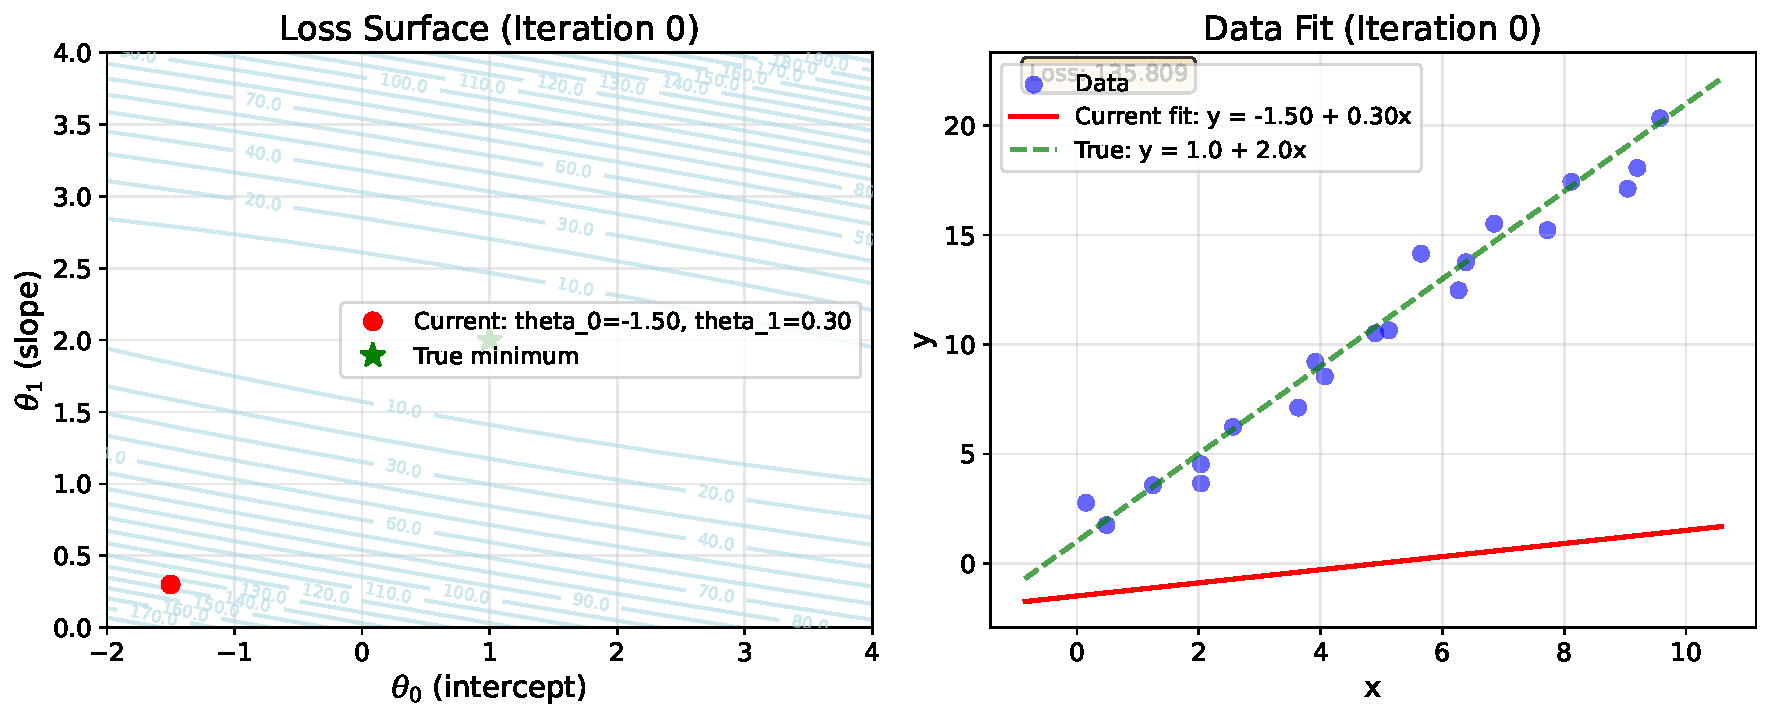
\includegraphics[scale=0.7]{../../maths/assets/mathematical-ml/figures/gradient-descent-0.pdf}}
    \only<2>{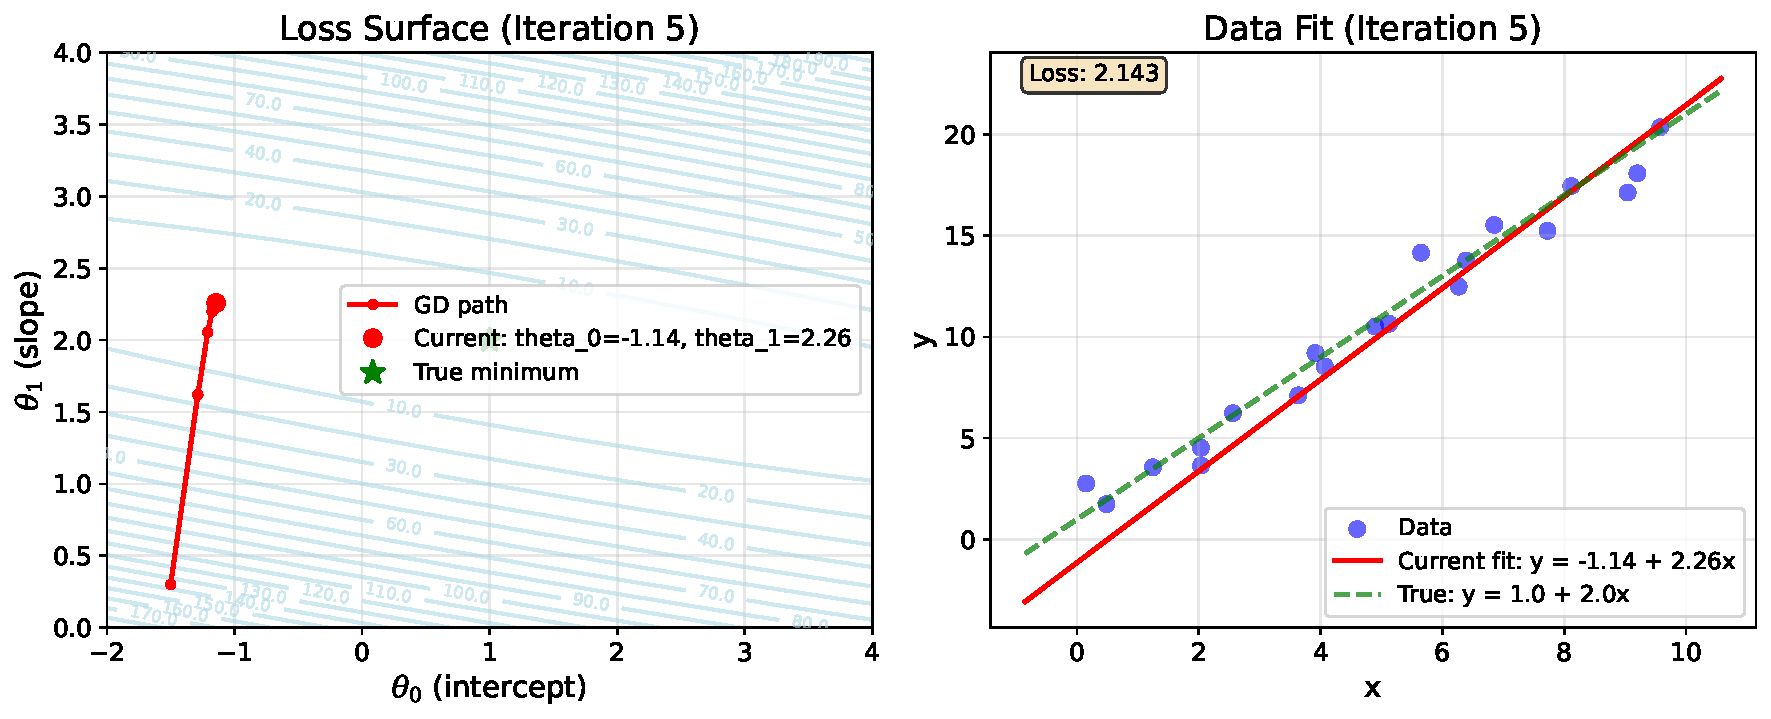
\includegraphics[scale=0.7]{../../maths/assets/mathematical-ml/figures/gradient-descent-5.pdf}}
    \only<3>{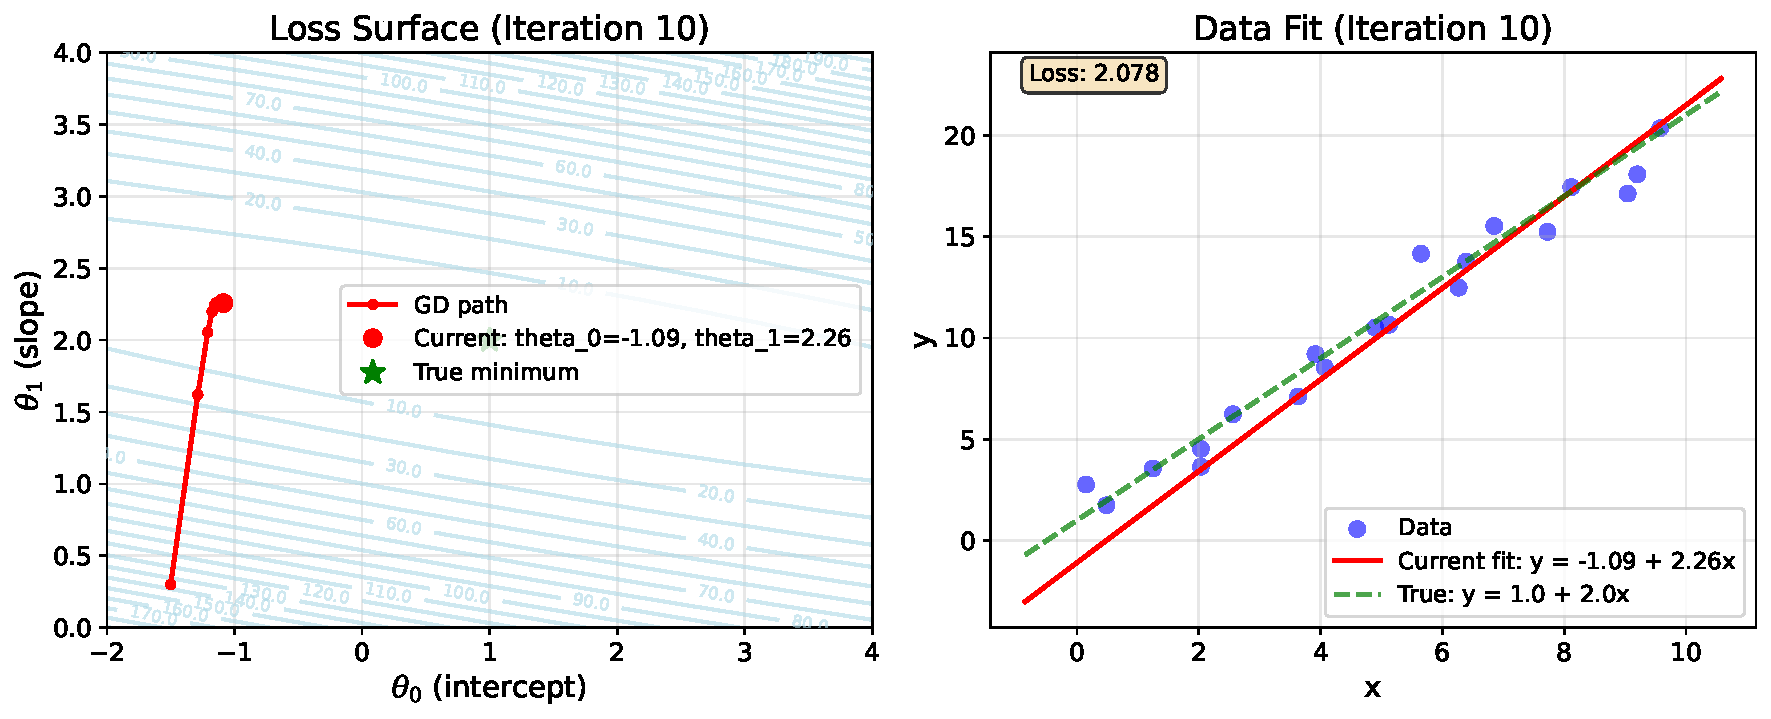
\includegraphics[scale=0.7]{../../maths/assets/mathematical-ml/figures/gradient-descent-10.pdf}}
    \only<4>{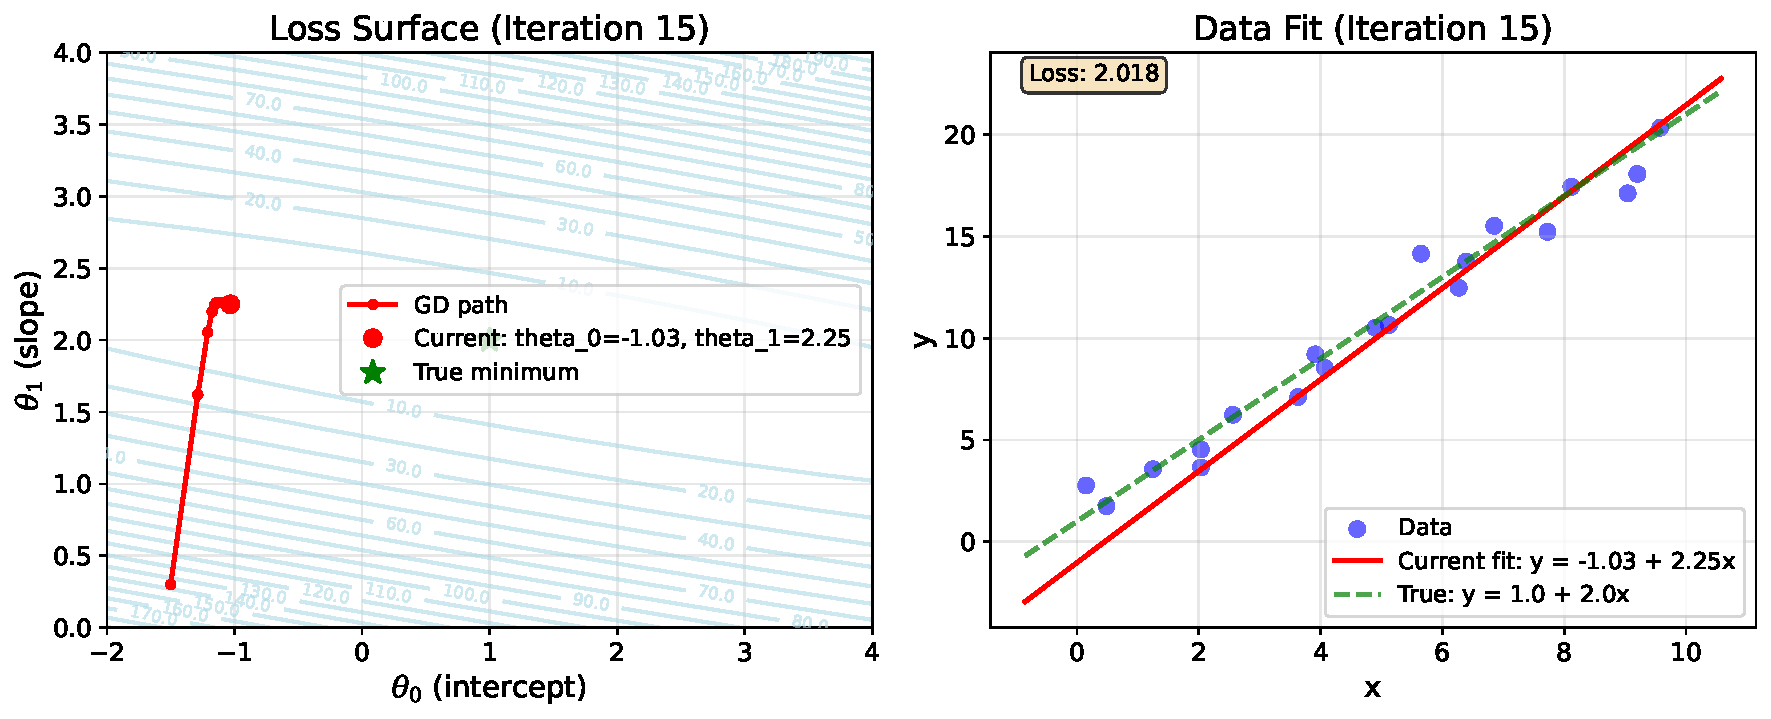
\includegraphics[scale=0.7]{../../maths/assets/mathematical-ml/figures/gradient-descent-15.pdf}}
    \only<5>{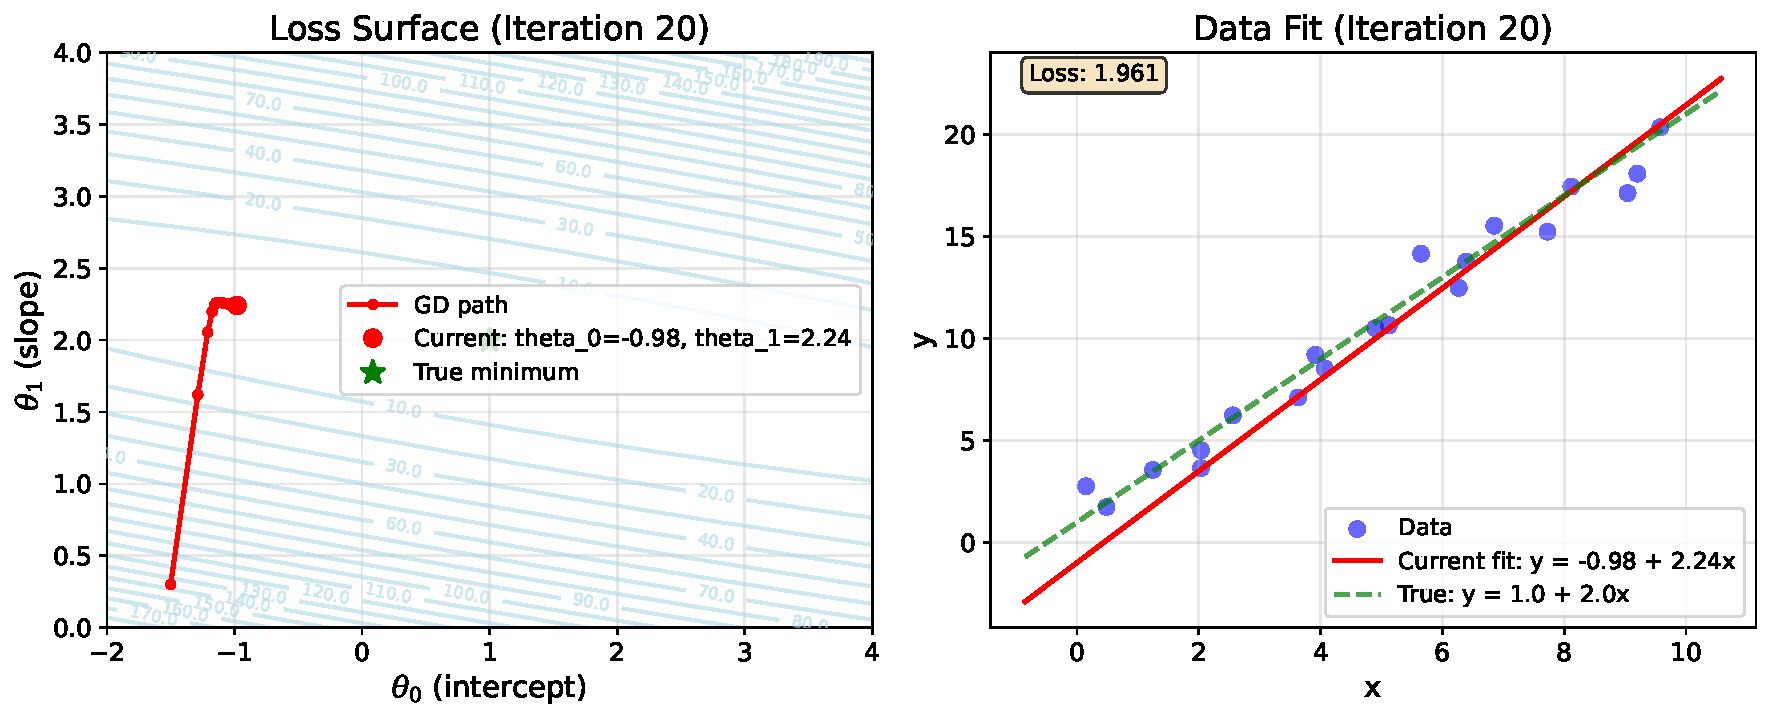
\includegraphics[scale=0.7]{../../maths/assets/mathematical-ml/figures/gradient-descent-20.pdf}}
    \end{center}
    
    \textbf{Notice:} The algorithm takes larger steps when gradient is large, smaller steps as it approaches the minimum!
  \end{frame}

  \begin{frame}{Loss vs. Iterations: Convergence Curves}
    % \begin{notebookbox}{https://nipunbatra.github.io/ml-teaching/notebooks/gradient-descent-2d.html}
    % Interactive gradient descent visualization and implementation
    % \end{notebookbox}
    
    \pause
    \textbf{What makes a good convergence curve?}
    \begin{itemize}[<+->]
        \item \textbf{Monotonic decrease:} Loss should never increase
        \item \textbf{Smooth convergence:} No wild oscillations
        \item \textbf{Plateau:} Eventually levels off at minimum
    \end{itemize}
    
    \pause
    \begin{alertbox}{Debug Tip}
    If your loss curve is noisy, jagged, or increasing, check your learning rate!
    \end{alertbox}
  \end{frame}

  \section{Variants of Gradient Descent}

  \begin{frame}{The Gradient Descent Family}
    \textbf{Three main variants based on how much data we use per update:}
    
    \begin{definitionbox}{Batch Gradient Descent (GD)}
    Use \textcolor{red}{all} training data to compute each gradient
    \end{definitionbox}
    
    \begin{definitionbox}{Stochastic Gradient Descent (SGD)}
    Use \textcolor{red}{one} sample to compute each gradient
    \end{definitionbox}
    
    \begin{definitionbox}{Mini-batch Gradient Descent (MBGD)}
    Use a \textcolor{red}{small batch} of samples to compute each gradient
    \end{definitionbox}
    
    \pause
    \textbf{Trade-offs:} Computational cost vs. convergence stability vs. memory usage
  \end{frame}

  \begin{frame}{Batch vs Stochastic vs Mini-batch}
    \begin{center}
    \begin{tabular}{|l|c|c|c|}
        \hline
        \textbf{Method} & \textbf{Data per update} & \textbf{Updates per epoch} & \textbf{Convergence} \\
        \hline
        Batch GD & $n$ (all) & 1 & Smooth \\
        \hline
        SGD & 1 & $n$ & Noisy \\
        \hline
        Mini-batch GD & $b$ (batch size) & $n/b$ & Balanced \\
        \hline
    \end{tabular}
    \end{center}
    
    \pause
    \begin{keypointsbox}
    \textbf{Modern ML:} Mini-batch GD with batch sizes 32-256 is most common
    \begin{itemize}
        \item Good balance of stability and efficiency
        \item Enables parallel computation (GPUs love batches!)
        \item Better gradient estimates than pure SGD
    \end{itemize}
    \end{keypointsbox}
  \end{frame}

  \begin{frame}{Stochastic Gradient Descent: The Noisy Path}
    \textbf{SGD uses one sample at a time for updates}
    
    \begin{center}
    \includegraphics[scale=0.5]{../../maths/assets/mathematical-ml/figures/gradient-descent-3-functions.pdf}
    \end{center}
    
    \pause
    \begin{itemize}[<+->]
        \item \textbf{Pro:} Fast updates, can escape local minima due to noise
        \item \textbf{Con:} Noisy convergence, may never reach exact minimum
        \item \textbf{Key insight:} The noise can be beneficial for non-convex problems!
    \end{itemize}
  \end{frame}

  \begin{frame}{Epochs vs Iterations: Important Distinction}
    \begin{definitionbox}{Iteration}
    One parameter update step (one gradient computation and update)
    \end{definitionbox}
    
    \begin{definitionbox}{Epoch}
    One complete pass through the entire training dataset
    \end{definitionbox}
    
    \pause
    \textbf{For dataset with 1000 samples:}
    \begin{itemize}[<+->]
        \item \textbf{Batch GD:} 1 iteration = 1 epoch
        \item \textbf{SGD:} 1000 iterations = 1 epoch  
        \item \textbf{Mini-batch (batch size 100):} 10 iterations = 1 epoch
    \end{itemize}
    
    \pause
    \begin{alertbox}{Important}
    Always report which metric you're using when discussing convergence speed!
    \end{alertbox}
  \end{frame}

  \section{Mathematical Properties}

  \begin{frame}{SGD as an Unbiased Estimator}
\textbf{True gradient:}\;
$\nabla L(\vtheta)=\tfrac{1}{n}\sum_{i=1}^n \nabla \ell(f(\vx_i;\vtheta),y_i)$

\pause
\textbf{SGD gradient estimate:}\;
$\nabla \tilde{L}(\vtheta)=\nabla \ell(f(\vx;\vtheta),y)$,
where $(\vx,y)$ is sampled uniformly from $\{(\vx_i,y_i)\}_{i=1}^n$.

\pause
\begin{theorembox}{Unbiased Estimator Property}
\[
\E[\nabla \tilde{L}(\vtheta)] = \nabla L(\vtheta)
\]
\end{theorembox}

\pause
\textbf{Proof:}
\begin{align*}
\E[\nabla \tilde{L}(\vtheta)]
&=\E\big[\nabla \ell(f(\vx;\vtheta),y)\big]\\
&=\sum_{i=1}^n \tfrac{1}{n}\,\nabla \ell(f(\vx_i;\vtheta),y_i)
= \nabla L(\vtheta).
\end{align*}
\end{frame}
  \begin{frame}{Why Unbiasedness Matters}
    \begin{keypointsbox}
    \textbf{Unbiased means:} On average, SGD points in the right direction!
    \end{keypointsbox}
    
    \pause
    \textbf{Implications:}
    \begin{itemize}[<+->]
        \item Individual SGD steps might be ``wrong'', but they average to the correct direction
        \item This theoretical guarantee justifies why SGD works in practice
        \item The noise in SGD can actually help escape local minima
    \end{itemize}
    
    \pause
    \begin{examplebox}{Intuitive Analogy}
    Imagine asking random people for directions to a destination:
    \begin{itemize}
        \item Individual answers might be slightly off
        \item But if there's no systematic bias, the average direction is correct
        \item SGD does the same with gradient estimates!
    \end{itemize}
    \end{examplebox}
  \end{frame}

  \section{Computational Complexity}

  \begin{frame}{Computational Complexity: GD vs Normal Equation}
    \textbf{For linear regression, we have two options:}
    
    \begin{alertbox}{Normal Equation}
    $\hat{\vtheta} = (\mX^T\mX)^{-1}\mX^T\vy$
    \\\textbf{Time complexity:} $\mathcal{O}(d^2n + d^3)$
    \end{alertbox}
    
    \begin{keypointsbox}{Gradient Descent}
    $\vtheta_{t+1} = \vtheta_t - \alpha \mX^T(\mX\vtheta_t - \vy)$
    \\\textbf{Time complexity:} $\mathcal{O}(T \cdot dn)$ for $T$ iterations
    \end{keypointsbox}
    
    \pause
    \textbf{When to use which?}
    \begin{itemize}[<+->]
        \item \textbf{Few features ($d$ small):} Normal equation
        \item \textbf{Many features ($d$ large):} Gradient descent
        \item \textbf{Non-linear models:} Only gradient descent works
    \end{itemize}
  \end{frame}

  \begin{frame}{Complexity Analysis: Breaking It Down}
    \textbf{Gradient Descent per iteration:}
    \begin{itemize}[<+->]
        \item Compute $\mX\vtheta$: $\mathcal{O}(nd)$ 
        \item Compute residual $\mX\vtheta - \vy$: $\mathcal{O}(n)$
        \item Compute $\mX^T$ (residual): $\mathcal{O}(nd)$
        \item Update $\vtheta$: $\mathcal{O}(d)$
        \item \textbf{Total per iteration:} $\mathcal{O}(nd)$
    \end{itemize}
    
    \pause
    \textbf{Normal Equation (one-time):}
    \begin{itemize}[<+->]
        \item Compute $\mX^T\mX$: $\mathcal{O}(d^2n)$
        \item Invert $\mX^T\mX$: $\mathcal{O}(d^3)$
        \item Compute $\mX^T\vy$: $\mathcal{O}(dn)$
        \item Final multiplication: $\mathcal{O}(d^2)$
        \item \textbf{Total:} $\mathcal{O}(d^2n + d^3)$
    \end{itemize}
  \end{frame}

  \stepcounter{popquiz}
  \begin{frame}{Pop Quiz \#\thepopquiz: Complexity Comparison}
    \begin{popquizbox}{\thepopquiz}
    You have a dataset with $n = 10^6$ samples and $d = 10^3$ features.
    
    \textbf{Questions:}
    \begin{enumerate}
        \item What's the complexity of normal equation?
        \item What's the complexity of 100 GD iterations?
        \item Which method would you choose and why?
        \item What if $d = 10^6$ instead?
    \end{enumerate}
    \end{popquizbox}
  \end{frame}

  \section{Advanced Topics and Extensions}

  \begin{frame}{Beyond Basic Gradient Descent}
    \textbf{Modern deep learning uses advanced optimizers:}
    
    \begin{itemize}[<+->]
        \item \textbf{Momentum:} $\vv_{t+1} = \beta \vv_t + (1-\beta)\vg_t$
        \item \textbf{AdaGrad:} Adaptive learning rates per parameter
        \item \textbf{Adam:} Combines momentum + adaptive learning rates  
        \item \textbf{RMSprop:} Exponential moving average of squared gradients
    \end{itemize}
    
    \pause
    \begin{examplebox}{Why These Improvements?}
    \begin{itemize}
        \item Handle different parameter scales automatically
        \item Accelerate convergence in relevant directions
        \item Reduce oscillations in narrow valleys
        \item Better performance on non-convex landscapes
    \end{itemize}
    \end{examplebox}
  \end{frame}

  \begin{frame}{Gradient Descent in Deep Learning}
    \begin{keypointsbox}
    Every modern deep learning framework uses gradient descent variants!
    \end{keypointsbox}
    
    \pause
    \textbf{Key extensions:}
    \begin{itemize}[<+->]
        \item \textbf{Backpropagation:} Efficient gradient computation for neural networks
        \item \textbf{Automatic differentiation:} PyTorch, TensorFlow handle gradients automatically
        \item \textbf{GPU acceleration:} Parallel computation of mini-batch gradients
        \item \textbf{Mixed precision:} Use both 16-bit and 32-bit arithmetic
    \end{itemize}
    
    \pause
    % \begin{notebookbox}{https://nipunbatra.github.io/ml-teaching/notebooks/}
    % Explore interactive examples of advanced optimizers in our notebook collection
    % \end{notebookbox}
  \end{frame}

  \section{Practical Considerations}

  \begin{frame}{Choosing Learning Rates: Practical Tips}
    \begin{keypointsbox}
    Learning rate selection is more art than science!
    \end{keypointsbox}
    
    \pause
    \textbf{Common strategies:}
    \begin{itemize}[<+->]
        \item \textbf{Grid search:} Try $\{0.001, 0.01, 0.1, 1.0\}$
        \item \textbf{Learning rate schedules:} Start high, decay over time
        \item \textbf{Adaptive methods:} Let the algorithm adjust automatically
        \item \textbf{Learning rate finder:} Gradually increase $\alpha$ and watch loss
    \end{itemize}
    
    \pause
    \begin{alertbox}{Warning Signs}
    \begin{itemize}
        \item Loss exploding $\rightarrow$ Learning rate too high
        \item Very slow convergence $\rightarrow$ Learning rate too low  
        \item Oscillating loss $\rightarrow$ Try smaller learning rate or momentum
    \end{itemize}
    \end{alertbox}
  \end{frame}

  \begin{frame}{Convergence Criteria: When to Stop?}
    \textbf{Common stopping criteria:}
    
    \begin{itemize}[<+->]
        \item \textbf{Gradient magnitude:} $||\nabla f(\vtheta)|| < \epsilon$
        \item \textbf{Function value change:} $|f(\vtheta_{t+1}) - f(\vtheta_t)| < \epsilon$
        \item \textbf{Parameter change:} $||\vtheta_{t+1} - \vtheta_t|| < \epsilon$
        \item \textbf{Maximum iterations:} Simple upper bound
    \end{itemize}
    
    \pause
    \begin{examplebox}{Practical Advice}
    \begin{itemize}
        \item Always set a maximum iteration limit
        \item Monitor multiple criteria simultaneously  
        \item Use validation set performance in practice
        \item Early stopping prevents overfitting
    \end{itemize}
    \end{examplebox}
  \end{frame}

  \begin{frame}{Common Pitfalls and How to Avoid Them}
    \begin{alertbox}{Pitfall 1: Poor Initialization}
    \textbf{Problem:} Starting at bad points (e.g., all zeros)
    \\\textbf{Solution:} Use Xavier/He initialization for neural networks
    \end{alertbox}
    
    \pause
    \begin{alertbox}{Pitfall 2: Learning Rate Too High/Low}
    \textbf{Problem:} Divergence or slow convergence
    \\\textbf{Solution:} Learning rate schedules, grid search, or adaptive optimizers
    \end{alertbox}
    
    \pause
    \begin{alertbox}{Pitfall 3: Poor Feature Scaling}
    \textbf{Problem:} Different parameter scales cause poor convergence
    \\\textbf{Solution:} Standardize features: $(x - \mu)/\sigma$
    \end{alertbox}
  \end{frame}

  \section{Summary and Key Takeaways}

  \begin{frame}{What We've Learned: The Big Picture}
    \begin{keypointsbox}
    Gradient descent is the foundation of modern machine learning optimization!
    \end{keypointsbox}
    
    \pause
    \textbf{Core concepts:}
    \begin{itemize}[<+->]
        \item \textbf{Mathematical foundation:} Taylor series approximation
        \item \textbf{Geometric intuition:} Follow steepest descent direction
        \item \textbf{Algorithm variants:} Batch, SGD, mini-batch
        \item \textbf{Theoretical properties:} SGD is unbiased estimator
        \item \textbf{Practical considerations:} Learning rates, convergence criteria
    \end{itemize}
  \end{frame}

  \begin{frame}{From Theory to Practice: Next Steps}
    % \begin{notebookbox}{https://nipunbatra.github.io/ml-teaching/notebooks/gradient-descent-2d.html}
    % Interactive gradient descent implementation and visualization
    % \end{notebookbox}
    
    \pause
    \textbf{Practice opportunities:}
    \begin{itemize}[<+->]
        \item Implement gradient descent from scratch
        \item Experiment with different learning rates
        \item Try different optimization functions
        \item Compare batch vs SGD vs mini-batch
        \item Visualize convergence paths
    \end{itemize}
  \end{frame}

  \stepcounter{popquiz}
  \begin{frame}{Pop Quiz \#\thepopquiz: Comprehensive Review}
    \begin{popquizbox}{\thepopquiz}
    \textbf{True or False?}
    \begin{enumerate}
        \item SGD always converges faster than batch gradient descent
        \item The learning rate should decrease as training progresses
        \item SGD gradient estimates are unbiased
        \item Normal equation is always better than gradient descent
        \item Gradient descent can only find global minima
    \end{enumerate}
    \end{popquizbox}
  \end{frame}

  \begin{frame}{Looking Ahead: Advanced Optimization}
    \textbf{What's next in optimization?}
    
    \begin{itemize}[<+->]
        \item \textbf{Second-order methods:} Newton's method, L-BFGS
        \item \textbf{Constrained optimization:} Lagrange multipliers, KKT conditions  
        \item \textbf{Global optimization:} Simulated annealing, genetic algorithms
        \item \textbf{Distributed optimization:} Federated learning, parameter servers
        \item \textbf{Meta-learning:} Learning to optimize
    \end{itemize}
    
    \pause
    \begin{keypointsbox}
    Master gradient descent first - it's the building block for everything else!
    \end{keypointsbox}
  \end{frame}

  % Include SGD notes
  \begin{frame}{Additional Resources: SGD Deep Dive}
    \begin{center}
    \textbf{For detailed mathematical analysis and proofs:}
    \end{center}
    
    % Include the SGD.pdf as reference
    \begin{alertbox}{Reference Material}
    See ``SGD.pdf'' in the assets folder for:
    \begin{itemize}
        \item Formal convergence proofs
        \item Variance analysis of SGD
        \item Advanced theoretical properties
        \item Comparison with other optimization methods
    \end{itemize}
    \end{alertbox}
    
    % \begin{notebookbox}{Additional Notebooks}
    % \begin{itemize}
    %     \item Gradient descent visualization: 2D and 3D examples
    %     \item Comparison of different optimizers
    %     \item Learning rate scheduling experiments
    %     \item Real-world optimization problems
    % \end{itemize}
    % \end{notebookbox}
  \end{frame}

  \begin{frame}
    \centering
    \Huge \textbf{Thank You!}
    
    \vspace{1cm}
    \Large Questions?
    
    \vspace{1cm}
    \normalsize
    \textbf{Next:} Advanced Optimization Techniques
    
    \textbf{Practice:} Implement gradient descent for your favorite ML model!
  \end{frame}

\end{document}